The data after preprocessing is clean from noise and other artifacts, now the most informative and distinguishing features are extracted for classification. This chapter discusses about different conventional feature extraction and classification methods that are widely researched in the BCI community. The methods discussed are implemented and compared on several basis in the following chapters. These methods are proven to be robust and applied to many existing BCI systems.

Researches such as \cite{2019_BMI_MIEEG} review various SOTA \nomenclature{SOTA}{State-of-the-art} signal processing pipelines for MI EEG based BCI systems. It discusses about different feature extraction, selection and classification techniques, and further about the benefits and challenges using them. 

\cite{2019_BMI_CARLA} studies integrating vehicle control systems (VCS) with 96-channels intra-cortical BCI and validated the concept with CARLA. The BCI signals were decoded and translated into acceleration, deceleration, turn right and turn left using a Python API. To demonstrate the potential of BCI for motion control of a car, a 1:10 scale remote controlled car was driven with the same commands offline. Several performance statistics were considered in evaluating the proposed methodologies.

\cite{2020_SP_comparison} provides a comparative study of various neuro-signal processing and classification methods.

\cite{2019_BCI_ROS} studies the integration of BCI systems with ROS-based control algorithms for navigation and obstacle avoidance to ease cognitive workload. The proposed algorithm is applied to a semi-autonomous navigation system where the BCI system decodes EEG commands to take a left or right turn and the direction information is used by ROS navigation stack to localize and move the robot with information also from different sensors and the provided static map.

\section{Feature Extraction} \label{feat_ext}
Brain signals are transient as well as diffuse spike and action potentials. They are rhythmic, hence could be sinusoidal or non-sinusoidal and includes small oscillations of semi periodic activation. \cite{2020_FeatExt_Review} reviews different feature extraction techniques for developing effective BCI system. Therefore the local information exists in time or frequency domain or both. \par

The brain signals could be time-locked i.e. the activity in the brain is time synchronized with the stimulus or the temporal dynamics is the same across every trial at the same instance. It could be phase-locked as well i.e. the phase angle time series is the same or similar on every trial. Depending on the type of the experiment used to gather data and the EEG paradigm, these parameters influence the choice of feature extraction mechanisms. 

In \cite{2022_MI_classification}, authors propose using statistical measures to extract features vector for motor imagery classfication task.

\subsection{Time Domain Analysis}
Time domain analysis is useful in extracting temporal features in the preprocessed measurement. Some of the commonly used time domain analysis methods include signal averaging, Hjorth parameters, fractal dimensions, auto regressive models, Bayesian filtering, Kalman filtering, particle filtering, zero crossing, template matching, power and window detection.\par

In case of non-phase locked brain signals, Time domain analysis leads to loss of information on averaging several trials but frequency analysis doesn't lose information on averaging trials.

\subsection{Frequency Domain Analysis}
Transforming the preprocessed data into frequency domain provides more useful information about the phase and amplitude of the brain signal required for analysis. Imagined movements lead to oscillations in premotor and sensorimotor areas, which is observed as amplitude changes in the $\mu$, $\beta$ and $\gamma$ region. These features can be used to create feature vectors. Some of the common frequency domain analysis are Fourier transform, Short-Time Fourier transform and Welch transform. These methods provide information on the spectral contents of the signal but not the temporal information of the event. 

\subsubsection{Fourier Transform (FT)}
Fourier transform decomposes signal into a weighted sum of sine and cosine waves of different frequencies. It works on the assumptions that the signal is infinite, periodic and stationary but brain signals do not hold to these assumptions. These shortcomings can be overcome by using short window periods for analysis, termed as Short-Time Frequency Transform (STFT) \nomenclature{STFT}{Short-Time Frequency Transform}. Another commonly used method for frequency domain analysis is Welch transform that provides smooth spectral decomposition. Phase content is not used in brain signal analysis in most cases as the signal could be non-phase locked. Hence amplitude information is mostly used in feature extraction. 

Power spectrum \ref{eq:pwr} obtained by square of amplitude in different frequency components during course of the task is the feature of interest in most BCI experiments.

\begin{equation} \label{eq:pwr}
    P(n) = A(n)^2
\end{equation}
where $A$ is the amplitude spectrum, $P$ is the Power Spectrum and $n$ denotes the index of the spectral bin.

\subsection{Time-Frequency Analysis (TFA)}
The method discussed above does not provide temporal information on occurrence of the event. Time-Frequency analysis on the signal provides temporal-spectral information. One of the most commonly used TFA method is wavelet transform.

\subsubsection{Wavelet Transform (WT)}
Wavelet transform uses finite basis functions called wavelets that are scaled and translated copies of finite length waveform called mother wavelet. Wavelets divide the signals of interest into different frequency components, each component can be studied at a resolution matched for its scale. A large scale component produces coarse resolution and small scale component produces fine resolution. The wavelet transform provides lower frequency resolution and higher temporal resolution at higher frequencies whereas higher frequency resolution and lower temporal resolution at lower frequencies. \par

\cite{2019_MI_MEWT} proposed a robust multivariate empirical wavelet transform algorithm for different Motor Imagery task.

Wavelet analysis is performed by convolution of wavelets of different scale and resolution with the signal of interest. The result of convolution contains components of the signal that are in the same frequency as the wavelet used. Scalogram provides a graphical way to interpret the time and frequency information of the signal. The transform could be either discrete or continuous depending upon the scale and translation parameters. Continuous Wavelet Transform (CWT) \nomenclature{CWT}{Continuous Wavelet Transform}provides more resolution than the Discrete Wavelet Transform (DWT)\nomenclature{DWT}{Discrete Wavelet Transform}.

A generic equation for a wavelet $\psi$ used in CWT can be written as \ref{eq:cwt}.

\begin{equation} \label{eq:cwt}
    \psi_{a,b}(t) = \frac{1}{\sqrt{a}} \psi( \frac{t - b}{a}) 
\end{equation}
where $t$ denotes time, $b$ is the shift parameter that slides the waveform along the time axis and $a$ is the scale factor that is used to scale the frequency of the wavelet.

Generally for a given wavelet function $\psi(\frac{t}{a})$ when $a > 1$ the mother wavelet dilates and it helps in capturing low frequency component and when $0 < a < 1$ it compresses the mother wavelet, capturing the high frequency components in the signal of interest. Thus $a \propto \frac{1}{f}$.

Wavelets have band-pass characteristics, with sum of all points being zero \ref{eq:wt_sum0} and its equivalent frequency can be determined by \ref{eq:wt_cf}.

\begin{equation} \label{eq:wt_sum0}
    \int\psi(t) dt = 0
\end{equation}

\begin{equation} \label{eq:wt_cf}
    F_{eq} = \frac{C_f}{a\delta_t}
\end{equation}
where $F_{eq}$ is the equivalent frequency, $C_f$ is the centre frequency, $a$ is the scaling factor and $\delta_t$ is the sampling interval.

A generic equation for a wavelet used in DWT can be written as \ref{eq:dwt}.

\begin{equation} \label{eq:dwt}
    \psi_{a,b}(t) = \frac{1}{2^{\frac{j}{v}}} \psi( \frac{n - m}{2^{\frac{j}{v}}}) 
\end{equation}
where $j$ is the scaling parameter, $v(>1)$ denotes voices per octave (logarithmic unit of ratio between two frequencies) and $m$ is the translational parameter.

% Table about wavelet scale

Various types of wavelets are used in research and one of the commonly used wavelet is the Morlet Wavelet. It the product of complex valued sine wave and Gaussian. In frequency domain, the amplitude spectrum of the complex morlet wavelet is not symmetrical and the power spectrum is independent of the phase relation between the wavelet and signal. The complex morlet wavelet can be written as \ref{eq:Mrlt1}.

\begin{equation} \label{eq:Mrlt1}
    \psi_\lambda(t) = e^{i2\pi ft -0.5(\frac{t}{\sigma})^2}
\end{equation}
where $\sigma = \frac{n}{2\pi f}$, $n$ is the number of cycles, $\lambda$ denotes a wavelet with specific scale and resolution parameters, $f$ is the frequency of the complex sine wave used.

The equation \ref{eq:Mrlt1} can also be written as  \ref{eq:Mrlt2}

\begin{equation} \label{eq:Mrlt2}
    \psi_\lambda(t) = e^{i2\pi ft} e^{-4\ln(2)\frac{t^2}{h^2}}
\end{equation}

A wavelet transform can be written as \ref{eq:WT_wx}.

\begin{equation} \label{eq:WT_wx}
    \mathcal{W}x  = \int x \ast \psi_\lambda(t) dt
\end{equation}

where $h$ is the full width half maximum (FWHM) \nomenclature{FWHM}{full width half maximum}parameter. With higher $n$, better temporal resolution and with lower $n$ better spectral resolution is achieved. Most algorithms work by starting with low number of cycles and gradually increasing to higher number of cycles. However the results of the wavelet convolution are easily interpretable only for stationary signals within the FWHM of the wavelet. With the right design of the wavelet this can be achieved.

\subsection{Wavelet Scattering Transform (WST)}
The wavelets are translated and convoluted with the signal of interest, as the wavelets commutes with translations the resulting expression becomes translation covariant. i.e. shifting the signal also shifts wavelet coefficients, therefore the comparison between translated signals becomes difficult. In order to make a proper representation of the signal the transform has to be translation invariant, stable under deformation and offer good structural information of all frequencies.

By WST\nomenclature{WST}{Wavelet Scattering Transform} non-informative variability in the signal such as translation, rotation and scaling are discarded. It can be suited for any application, with more data a pre-trained model is used as a pipeline and for small datasets wavelet scattering initialization could be performed. WST yields representations that are translation invariant and stable against time warping deformations. This is achieved by subsequent non-linearity and averaging steps after convolving with the wavelet. 

As EEG signals can be influenced and varied by various factors Electrocardiography(ECG) provides more stable signals that can be used for analysis. In \cite{2021_ECG_WST_ML}, the author performs emotion recognition from ECG signals using WST for feature extraction and evaluated the system for several classifiers.

CWT is the basic building block for WST. CWT measures similarity of the signal with wavelets of varying frequency and scale at each point in time. For a given wavelet $\psi$, it is first shifted by time $\tau$, the similarity if found by computing the inner product $\left\langle x, \psi \right\rangle$. This is repeated for all $\tau$ and $\psi$.

Any linear operation which is translation invariant of a wavelet coefficient will result in zero, which is not informative. Hence a non-linear invariant operand is required. Modulus being a non-linear, optimal contractive operator, when applied on CWT as given in \ref{eq:wst_TI}, removes the phase information in the signal and makes it invariant to translations. This gives a measure on sparsity of the wavelet coefficients. The coefficients obtained are called as unaveraged coefficients. 

\begin{equation} \label{eq:wst_TI}
    \begin{split}
     \mathcal{U} x = |\mathcal{W} x|\\
     \int | x \ast \psi_\lambda(t) | dt = \| x \ast \psi_{\lambda_{1}}\|_1 
    \end{split}
\end{equation}
where $\lambda_1 = 2^j$ is the centre frequency of the first order wavelets, with $j$ scale factor.

The unaveraged coefficients when convolved again with a low-pass or scaling filter(also called father wavelet) $\phi$ as given in \ref{eq:wst_def} performs temporal averaging of the signal. The coefficients obtained are called Scattering coefficients. It imposes stability against time warping deformations. This however removes high frequency information, but can be recovered by performing WST again on the unaveraged coefficients.

\begin{equation} \label{eq:wst_def}
    \begin{split}
        \mathcal{S} x = \mathcal{U} x \ast \phi\\
        \mathcal{S} x(t, \lambda_1) = \| x \ast \psi_{\lambda_{1}}\|_1 \ast \phi         
    \end{split}
\end{equation}

The above steps are performed recursively (usually 3 orders) on the results on the unaveraged coefficients and the features are extracted at each level by convolving the results with low-pass filter. Scatter representations consists of {0,1,2} order coefficients which are generated by composing wavelets in different sequences. Multiple wavelets composed together called filter banks, capture high frequency components. Each filter bank consists of several dilated and rotated wavelets with no orthogonality.

Consider family of wavelets ${\psi_{\lambda}}$. The dilated wavelet can be written as \ref{eq:wst_dila}

\begin{equation} \label{eq:wst_dila}
    \psi_{\lambda}(t) = 2^{\frac{-j}{Q}}\psi(2^{\frac{-j}{Q}}t)
\end{equation}
where $Q$ is number of band-pass filter in an octave.

\begin{equation} \label{eq:wst_wt}
    \mathcal{W} x = \{x\ast \phi(t) , x\ast \psi_\lambda(t) \}
\end{equation}

The second order coefficients obtained can be decorrelated to increase their invariance through renormalization. Different features are obtained at each order of coefficients. The first order coefficients represents the frequency content (oscillation rate) in the signal, the second order coefficients represents rates of frequency change, treat every rate from first order as its own signal and repeat first order upon each modulus. 

 \subsubsection{Exponential decay of scattering coefficients}
 Repeated application of modulo moves the energy contained in the high frequencies of the initial signal towards low frequencies. Convolution with the low-pass filter picks that energy and uses it in  feature extraction. At each step of the scattering transform, energy in the lowest frequency bands is output by convolution with a low-pass filter at its respective step. The remaining part of the energy is shifted towards the lower frequencies by applying modulus of wavelet transform.
 
 \begin{equation} \label{eq:wst_wt1}
    \mathcal{W} x = \{x\ast \phi(t) , x\ast \psi_\lambda(t) \} \\
\end{equation}

If $|\hat{\phi}(w)|^2 + \sum_{\lambda} | \hat{\psi}_{\lambda}(w)|^2 = 1$ then $\mathcal{W}$ is unitary.

\begin{equation}    
    \|\mathcal{W}x\|^2 = \|x\ast\phi\|^2 + \sum_{\lambda}\| x \ast \psi_\lambda\| = \|x\|^2
\end{equation}

\subsubsection{Neural Network representation of WST}
 Typical Convolutional Neural Network (CNN) \nomenclature{CNN}{Convolutional Neural Network} involves, successive operations involving convolution, non-linearity, pooling/sub-sampling. WST performs the same operations, hence WST can be represented as a neural network called Wavelet Scattering Network (WSN) \nomenclature{WSN}{Wavelet Scattering Network} to extract the scattering coefficients. This can be highly efficient as the wavelets values for the filter bank are predetermined hence learning is not required and no complex architecture has to be designed. Kymatio \cite{2020_kymatio}is an open-source WST implementation that leverages machine learning framework like PyTorch, Keras or Scikit-learn in the back-end.

\subsection{Spatial Analysis}
The spatial filters invert the measurement to its original source. Spatial Analysis helps in mapping the source signals to the brain topography that can be used for further topographical studies. In general \textit{Patterns} are not \textit{Filters}. Patterns denote the propagation of a source to sensors which are used in forward model \ref{eq:fwd_model}. Filters on the other hand denote weighting of EEG channels and are used in backward model \ref{eq:bck_model} to extract individual components.

\begin{equation} \label{eq:fwd_model}
    x(t) = A s(t) +n(t)
\end{equation}
where $s$ can be a vector denoting sources. $n$ is a noise vector and $x$ is the measurement at the channel. A is the forward or mixing matrix in which every column corresponds to a spatial pattern.

\begin{equation} \label{eq:bck_model}
    \hat{s}(t) = W^T x(t)
\end{equation}
where $W$ represents the unmixing matrix where every row of $W^T$ corresponds to spatial filter.

The spatial map of a filter is hard to interpret, but patterns are easy to interpret and hence patterns corresponding to a given spatial filter is found.

\subsubsection{Common Spatial Patterns (CSP)}
CSP \nomenclature{CSP}{Common Spatial Patterns}is a supervised feature extraction method for classification algorithms which works only for motor-imagery information in EEG. It learns to optimally discriminate band power features using multiple electrodes placed at optimal regions. Variance of the band pass signal is proportional to the band power of the frequency band. CSP leverages this by finding patterns where the  variance of filtered data from one class is maximized while variance of filtered data from other class is minimized. The resulting feature vector enhances discriminability between different classes. However it works on the assumptions that frequency band and time window of the measurements are known, source activity constellation differs between two classes and the band passed signal is jointly Gaussian within the time window. Such patterns and filters obtained from OpenBCI headgear is given in \ref{fig:obci_csp_pat} and \ref{fig:obci_csp_filt}.

\cite{2022_CSP_RiemGeo_Errp} proposed a statistical spatial filter that enables cross-session and cross-subject generalization thus avoiding re-calibration for every session or every subject. 

\cite{2019_FBCSP_FeatGen} proposed a channel selection method for extracting motor imagery features using filter-bank common spatial pattern.

\begin{figure}[H] 
    \begin{center}
    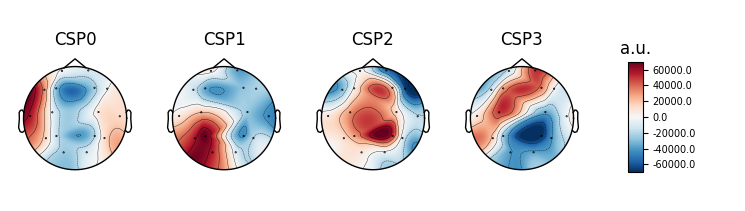
\includegraphics[width=1.0\textwidth]{images/obci_csp_pat.png}
    \caption{CSP Patterns obtained from OpenBCI EEG data}
    \label{fig:obci_csp_pat}
\end{center}
\end{figure}

\begin{figure}[H] 
    \begin{center}
    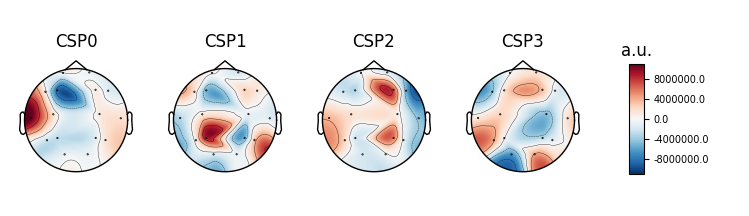
\includegraphics[width=1.0\textwidth]{images/obci_csp_filt.png}
    \caption{CSP Filters obtained from OpenBCI EEG data}
    \label{fig:obci_csp_filt}
\end{center}
\end{figure}

\cite{2017_EEGChannelSelection} studies different variants of CSP that could achieve maximum accuracy with least number of EEG channels. This helps removing noisy channels and avoid over-fitting. The study revealed that a conventional CSP without any regularization applied performs better on cross-subject validation. \cite{2017_MI_ML_SP} proposed motor imagery classification pipeline using channel selection, band passing and  CSP based extraction of 38 features and Gaussian Naive Bayes (GNB) classifier.

Consider measurement data set $\{\mathbb{X}^{i}_{c}\}^{k}_{i=1}$ for trial $i$ belonging to class $c \in\{1,2\}$. Each $\{\mathbb{X}^{i}_{c}\}$ is a $N * T$ matrix, where N is the number of channels and T is the number of samples per channel. The goal of CSP is to find $W$ given by $N * M$, consisting M spatial filters i.e. each column is a  spatial filter, that transforms the measured signals \ref{eq:trans_csp}.

\begin{equation} \label{eq:trans_csp}
    x_{CSP}(t) = W^{T}x(t)
\end{equation}
where $x(t)$ is vector of input signals at time $t$ from all channels. CSP can formally be defined for a two class problem as \ref{eq:def_csp}.

\begin{equation} \label{eq:def_csp}
    \begin{split}
        J(w) = \frac{WX_{1}X_{1}^TW^T}{WX_{2}X_{2}^TW^T} \\
         = \frac{WC_{1}W^T}{WC_{2}W^T}
    \end{split}
\end{equation}
where $C_{c}$ is the spatial covariance matrix for class $c$, $W$ is the spatial filter to optimize and $X_{c}$ is the multichannel EEG signal from class $c$. The problem could be solved to either minimize $J(w)$ where variance in $X_{1}$ is minimized and maximized in $X_{2}$ or maximize $J(w)$ where variance in $X_{1}$ is maximized and minimized in $X_{2}$.

This can be computed by Generalized Eigen Value Decomposition (GEVD) of $C_{1}$ and $C_{2}$. The Eigen vectors corresponding to the largest eigen value will maximize $J(w)$ and eigen vectors corresponding to the smallest eigen value will minimize $J(w)$. 

\begin{equation} \label{eq:def_csp}
    \begin{split}
        WC_{1}W^T = \Lambda_{1}\\
        WC_{2}W^T = \Lambda_{2}
    \end{split}
\end{equation}
where  $\Lambda_{1}$ and  $\Lambda_{2}$ are diagonal matrices containing eigen values such that $\Lambda_{1} + \Lambda_{2} = \mathbf{I}$

\begin{equation} \label{eq:def_gevd}
    WC_{1}W^T = \Lambda W^T(C_{1} + C_{2})W = \mathbf{I}
\end{equation}

Typically 3 CSP filter pairs i.e. minimization and maximization are used which results in 6 feature vectors that forms the filter matrix $W$. Once the filter is obtained, the prediction function using CSP can be defined as \ref{eq:feat_csp}.

\begin{equation} \label{eq:feat_csp}
    \begin{split}
    y = sign(\theta log(var(WX)) +b) \\
        = sign(\theta log(WCW^T) + b)
    \end{split}
\end{equation}
The application of log on the spatially filtered data makes it a Gaussian distribution. The classifier applied can be either linear or nonlinear. After applying CSP the data is rotated and placed orthogonal.

CSP is simple, computationally efficient with high classification performance. But it is not robust to noise and non-stationarity, prone to over-fitting and requires many training examples. Several variants of CSP are researched and developed such as Filter Bank CSP, Regularized CSP and Invariant CSP to overcome the disadvantages of vanilla CSP.

% \section{Feature Selection} 

\section{Classification} \label{clasff}
With the required features extracted, the vectors can be forwarded to the classifier as a last step in the BCI pipeline. Some of the most commonly used classifiers include SVM, LDA\dots These could also be neural networks, but a neural network could also perform feature extraction, hence it would not be efficient to use a neural network just for classification. However several literature have used neural networks only as a classifier.
\cite{2004_EEG_ML} discusses the machine learning methods, their application to BCI, and validating them for BCI. It discusses about SVM and how regularization is beneficial for BCI data. In case of nonlinear data, it can be converted to a linearly separable feature space and efficiently used for classification without any complexity. \cite{2006_EEG_ML_BrainState} discusses about how machine learning is applied to motor imagery with feedback.

\subsection{Support Vector Machines (SVM)}
SVM \nomenclature{SVM}{Support Vector Machine}is the most commonly used classifiers as they provide highly accuracy with less compute power. The aim of SVM as a classifier is to find the hyperplane such that it separates the support vectors with a high margin. 
In \cite{2018_BCI_SVM_DNN} and \cite{2021_Feat_MI_TF_ICA_SVM}, SVMs were used at the end of the BCI processing pipeline to classify the motor intent of the user.

\subsection{Linear Discriminant Analysis (LDA)}
LDA \nomenclature{LDA}{Linear Discriminant Analysis} is considered to be optimal classifier given the following assumptions are true:
\begin{enumerate}
    \item Features of each class are Gaussian distributed.
    \item Gaussian's of all classes have the same covariance matrix.
    \item True class distributions are known.
\end{enumerate}

Given two class distributions $\mathcal{N} (\mu_1, \epsilon )$ and $\mathcal{N} (\mu_2, \epsilon  )$ , then LDA is defined by normal vectors

\begin{equation} \label{eq:lda_w}
    \begin{split}
        w = \epsilon^{-1} (\mu_2 - \mu_1)
    \end{split}
\end{equation}
and
\begin{equation} \label{eq:lda_b}
    \begin{split}
        b = w^T(\mu_2 + \mu_1)/2
    \end{split}
\end{equation}

 But as the true class distribution is not known, the distributions are estimated, which is usually different from the true value  and it determines the performance of the classifier. Shrinkage-LDA overcomes this problem by using a shrunk covariance matrix that is determined by optimal shrinkage parameter given by analytical and cross-validation methods.

\section{Summary}
The right choice of feature extraction methods and classifiers depends on the EEG paradigm used and features of interest as different features extraction methods provide different aspects of the EEG signal. The feature extraction and classification methods discussed in this chapter provides rich information on various aspects of the signal. Time-Frequency analysis provides spatio-temporal information, which helps in extraction several rich features. In particular, WST backed with neural network can classify the brain signals without the need to learn the filter co-efficients.  With enough labelled data, CSP algorithms are simple and effective in classification of motor imagery information. SVM are the most researched and widely applied classifier for a BCI system. However the pipeline setup with the above discussed methods is very task specific and it requires reestablishing the pipeline for a different application. The next chapter discusses about how some deep learning techniques provide a generic system for several applications with minimal tuning.